% =============================================================================
%  Atto 4 — The Downstream Path  (~15 min, ~10 slide)  [Parte II.A]
%  Spine of the talk: a single cmd_vel followed all the way to a transistor.
% =============================================================================

\section{Part II.A — Downstream: a \texttt{cmd\_vel}, end to end}

% ---------------------------------------------------------------------------- %
\begin{frame}{Lighting the path we are about to walk}
  \begin{columns}[T,onlytextwidth]
    \column{0.55\textwidth}
      
\includegraphics[width=\linewidth]{MiviaRoverLogicalView.png}

    \column{0.40\textwidth}
      \textbf{Five rings, walked one at a time.}
      \vspace{0.6em}

      \begingroup
      \setlength{\tabcolsep}{0pt}
      \renewcommand{\arraystretch}{1.25}
      \begin{tabular}{@{}p{10mm}@{\hspace{2mm}}p{48mm}@{}}
        \textcolor{Accent}{\scriptsize\bfseries Ring 1} &
          \texttt{diff\_drive\_controller}\\[-1pt]
        & \scriptsize\textcolor{black!60}{kinematics}\\[2pt]

        \textcolor{Accent}{\scriptsize\bfseries Ring 2} &
          URDF \texttt{<ros2\_control>}\\[-1pt]
        & \scriptsize\textcolor{black!60}{contract toward the host}\\[2pt]

        \textcolor{Accent}{\scriptsize\bfseries Ring 3} &
          Custom \texttt{MiviaRoverSystem}\\[-1pt]
        & \scriptsize\textcolor{black!60}{lifecycle, RT buffers, comm thread}\\[2pt]

        \textcolor{Accent}{\scriptsize\bfseries Ring 4} &
          ROS-side CAN stack\\[-1pt]
        & \scriptsize\textcolor{black!60}{\texttt{ros2\_socketcan} + parser}\\[2pt]

        \textcolor{Accent}{\scriptsize\bfseries Ring 5} &
          Bring-up \& launch order\\[-1pt]
        & \scriptsize\textcolor{black!60}{\texttt{controller\_manager} + spawners}
      \end{tabular}
      \endgroup
  \end{columns}
\end{frame}

% ---------------------------------------------------------------------------- %
\begin{frame}{ros2\_control, only what we need to know}
  \begin{columns}[T,onlytextwidth]
    \column{0.50\textwidth}
      \textbf{One process: \texttt{ros2\_control\_node}.}
      \begin{itemize}\setlength\itemsep{1pt}
        \item Runs the \texttt{controller\_manager}, which owns a
              \texttt{ResourceManager}.
        \item Loads each \textbf{hardware component} as a plugin and
              exposes its \emph{state} and \emph{command} interfaces.
        \item A fixed-rate loop calls, on every tick:\\[1pt]
              \makebox[\linewidth][c]{%
                \(\texttt{read()}\!\to\!\texttt{ctrl.update()}\!\to\!\texttt{write()}\)}
        \item That rate is the \textbf{system clock} of the control side.
      \end{itemize}

      \vspace{0.3em}
      \footnotesize\alert{We ignore the rest:} controller chains, mode
      switching, claiming policies. The four bullets above are all you
      need to build a minimal platform interface.

    \column{0.45\textwidth}
      \textbf{Lifecycle of every hardware component.}\\[1pt]
      \centering
      \begin{tikzpicture}[
        node distance=3.5mm,
        every node/.style={font=\scriptsize},
        life/.style={hl, minimum width=28mm, minimum height=6.5mm},
        lifearr/.style={arrhl, line width=0.65pt,
          -{Latex[length=1.7mm,width=1.3mm]}, shorten <=0.8mm, shorten >=0.8mm}
      ]
        \node[life]                (init){\texttt{on\_init}};
        \node[life, below=of init] (cfg) {\texttt{on\_configure}};
        \node[life, below=of cfg]  (act) {\texttt{on\_activate}};
        \node[life, below=of act]  (run) {\texttt{read()/write()}};
        \node[life, below=of run]  (deact){\texttt{on\_deactivate}};
        \node[life, below=of deact](cln) {\texttt{on\_cleanup}};
        \draw[lifearr] (init.south)-- (cfg.north);
        \draw[lifearr] (cfg.south) -- (act.north);
        \draw[lifearr] (act.south) -- (run.north);
        \draw[lifearr] (run.south) -- (deact.north);
        \draw[lifearr] (deact.south)-- (cln.north);
      \end{tikzpicture}\\[2pt]
      \scriptsize\textcolor{black!60}{Resources allocated in
      \texttt{on\_configure}; \texttt{on\_init} only validates.}
  \end{columns}
\end{frame}

% ---------------------------------------------------------------------------- %
\begin{frame}[fragile]{Ring 1 — \texttt{diff\_drive\_controller}}
  \begin{columns}[T,onlytextwidth]
    \column{0.45\textwidth}
      \textbf{What it consumes.} A \texttt{TwistStamped} on \texttt{cmd\_vel} topic.

      \textbf{What it produces.} A \emph{velocity} command on \emph{four}
      command interfaces — one per wheel joint.

      \textbf{Why it works for our 4WD skid-steer.} We group the wheels
      \emph{two by two} and tell the controller it is a 2-side differential
      drive. Slip is absorbed at the firmware level.

      \vspace{0.4em}
      \footnotesize\textcolor{black!60}{Same controller does inverse \emph{and}
      forward kinematics — odometry comes back for free in Atto~5.}

    \column{0.5\textwidth}
      \begin{lstlisting}[language=, basicstyle=\ttfamily\scriptsize]
mivia_rover_base_controller:
  ros__parameters:
    left_wheel_names:
      ["wheel_fl_joint", "wheel_rl_joint"]
    right_wheel_names:
      ["wheel_fr_joint", "wheel_rr_joint"]

    wheel_separation: 0.355   # [m]
    wheel_radius:     0.085   # [m]
    wheels_per_side:  2

    publish_rate: 50.0
    cmd_vel_timeout: 0.5
      \end{lstlisting}
      \scriptsize\textcolor{black!60}{\texttt{mivia\_rover\_controllers.yaml}
      — geometry must match the URDF.}
  \end{columns}
\end{frame}

% ---------------------------------------------------------------------------- %
\begin{frame}[fragile]{Ring 2 — the URDF \texttt{<ros2\_control>} block}
  \begin{columns}[T,onlytextwidth]
    \column{0.45\textwidth}
      \textbf{The contract \emph{toward} ros2\_control.}\\
      \small Each wheel exposes one command and two state signals.

      \vspace{0.5em}
      \begingroup
      \setlength{\tabcolsep}{0pt}
      \renewcommand{\arraystretch}{1.2}
      \begin{tabular}{@{}p{15mm}@{\hspace{2mm}}p{35mm}@{}}
        \textcolor{Accent}{\scriptsize\bfseries command} &
          \texttt{velocity}\\[-1pt]
        & {\scriptsize\textcolor{black!60}{written by the controller}}\\[3pt]

        \textcolor{Accent}{\scriptsize\bfseries state} &
          \texttt{position} \(+\) \texttt{velocity}\\[-1pt]
        & {\scriptsize\textcolor{black!60}{filled by the SystemInterface}}
      \end{tabular}
      \endgroup

      \vspace{0.8em}
      \textbf{The \texttt{<plugin>} selects the class.}\\
      \small \texttt{MiviaRoverSystem} is loaded by the
      \texttt{ResourceManager} through \texttt{pluginlib}.

      \vspace{0.5em}
      {\scriptsize\textcolor{black!60}{Inline hardware parameters are forwarded
      once, at \texttt{on\_init}.}}

    \column{0.50\textwidth}
      \begin{lstlisting}[language=XML, basicstyle=\ttfamily\scriptsize,
                         keywordstyle=\color{HLOrange}]
  <hardware>
    <plugin>
      mivia_rover_platform/MiviaRoverSystem
    </plugin>
    <param name="encoder_topic">
      /mivia_rover/encoder_rpms</param>
    <param name="reference_topic">
      /mivia_rover/reference</param>
    <param name="fb_timeout_ms">150</param>
    <param name="rpm_limit_abs">180</param>
    <param name="publish_rate_hz">50</param>
  </hardware>

  <joint name="wheel_fl_joint">
    <command_interface name="velocity"/>
    <state_interface   name="position"/>
    <state_interface   name="velocity"/>
  </joint>
  ...  <!-- fr / rl / rr -->
</ros2_control>
      \end{lstlisting}
  \end{columns}
\end{frame}

% ---------------------------------------------------------------------------- %
\begin{frame}{Ring 3 — anatomy of a custom \texttt{SystemInterface}}
  \begin{columns}[T,onlytextwidth]
    \column{0.45\textwidth}
      \textbf{Why custom.}\;
      Our CAN protocol is custom, so the rover implements
      \texttt{hardware\_interface::SystemInterface} directly.

      \textbf{What we override.}
      \begin{itemize}\setlength\itemsep{1pt}
        \item \texttt{on\_init} — params, joints, buffers.
        \item \texttt{on\_configure} — ROS node + \emph{comm thread}.
        \item \texttt{export\_*} — expose state/command buffers.
        \item \texttt{read} / \texttt{write} — control-loop boundary.
      \end{itemize}

    \column{0.50\textwidth}
      \centering
      \begin{tikzpicture}[
        node distance=7mm,
        sysnode/.style={minimum width=54mm, minimum height=8mm},
        sysarr/.style={line width=0.65pt,
          {Latex[length=1.8mm,width=1.4mm]}-{Latex[length=1.8mm,width=1.4mm]},
          shorten <=1mm, shorten >=1mm}
      ]
        \node[hl, sysnode] (cm)
              {\texttt{controller\_manager} (RT thread)};
        \node[hl, sysnode, below=of cm] (sys)
              {\textbf{MiviaRoverSystem}\\\scriptsize state $\leftarrow$ \texttt{readFromRT()};\;cmd $\to$ buffer};
        \node[bus, sysnode, below=of sys] (rtb)
              {RT buffers + lock-free double-buffer};
        \node[ll, sysnode, below=of rtb] (comm)
              {Comm thread (NON-RT)\\\scriptsize ROS pub/sub at \(50\)~Hz};

        \draw[arrhl, sysarr] (cm.south) -- (sys.north);
        \draw[arrhl, sysarr] (sys.south) -- (rtb.north);
        \draw[arrll, sysarr] (rtb.south) -- (comm.north);
      \end{tikzpicture}\\[2pt]
      \scriptsize\textcolor{black!60}{Hard real-time on top, ROS comm at
      the bottom, wait-free buffers in the middle.}
  \end{columns}
\end{frame}

\begin{comment}
% ---------------------------------------------------------------------------- %
\begin{frame}[fragile]{Ring 3.b — \texttt{write()} in detail}
  \begin{columns}[T,onlytextwidth]
    \column{0.50\textwidth}
      \texttt{write()} receives four wheel setpoints in
      \texttt{hw\_commands\_}.

      \vspace{0.3em}
      Its job is deliberately small:
      \begin{enumerate}\setlength\itemsep{2pt}
        \item convert rad/s \(\to\) RPM,
        \item clamp to \texttt{rpm\_limit\_abs},
        \item publish a sample for the comm thread.
      \end{enumerate}

      \vspace{0.5em}
      \textbf{Lock-free double-buffer.}\\
      \small RT writes the next slot and advances an atomic
      \texttt{seq}; the comm thread snapshots the published slot by value.

      \vspace{0.4em}
      \alert{No mutex:} \small the control loop must not wait for ROS
      publishing.

    \column{0.45\textwidth}
      \begin{lstlisting}[language=C++, basicstyle=\ttfamily\scriptsize]
// Pseudocode
// RT-safe publish to comm thread
CommandSample c;
c.stamp_ns = time.nanoseconds();
for (k = 0..3)
  c.rpm[k] = clamp_rpm(
      rad_s_to_rpm(hw_commands_[k]),
      rpm_limit_abs);

uint32_t seq = cmd_seq_.load(relaxed);
size_t   next_idx = (seq + 1) & 1;
cmd_buf_[next_idx] = c;
cmd_valid_.store(true,  release);
cmd_seq_.store(seq + 1, release);
      \end{lstlisting}
      \scriptsize\textcolor{black!60}{\textit{actual code from
      \texttt{mivia\_rover\_system.cpp:519--546}}}
  \end{columns}
\end{frame}

% ---------------------------------------------------------------------------- %
\begin{frame}[fragile]{Ring 3.c — the comm thread}
  \begin{columns}[T,onlytextwidth]
    \column{0.50\textwidth}
      The comm thread runs outside the RT loop, at \(50\)~Hz.

      \vspace{0.3em}
      Each tick:
      \begin{enumerate}\setlength\itemsep{2pt}
        \item drain incoming \texttt{EncoderRpms},
        \item snapshot the latest command sample,
        \item replace it with zeros on \texttt{fault\_stop\_},
        \item publish one \texttt{Reference}.
      \end{enumerate}

      \vspace{0.5em}
      \alert{Never go silent:} \small even a stop is an explicit CAN
      reference.

      \vspace{0.4em}
      \textbf{Why publish?}\\
      \small Ring~4 owns CAN serialization and transport through
      \texttt{ros2\_socketcan}.

    \column{0.45\textwidth}
      \begin{lstlisting}[language=C++, basicstyle=\ttfamily\scriptsize]
// Pseudocode comm thread, 50 Hz
while (comm_running_) {
  exec_->spin_some();
  Reference out;
  out.header.stamp = node->now();

  if (fault_stop_) {
    out.front_left  = 0;
    out.rear_left   = 0;
    out.front_right = 0;
    out.rear_right  = 0;
  } else {
    seq = cmd_seq_.load(acquire);
    snapshot = cmd_buf_[seq & 1];
    out.front_left  = snapshot.rpm[0];
    out.rear_left   = snapshot.rpm[1];
    out.front_right = snapshot.rpm[2];
    out.rear_right  = snapshot.rpm[3];
  }
  reference_pub_->publish(out);
  sleep_for(1/hz);
}
      \end{lstlisting}
  \end{columns}
\end{frame}
\end{comment}

% ---------------------------------------------------------------------------- %
\begin{frame}{Ring 4 — the ROS-side CAN stack}
  \centering
  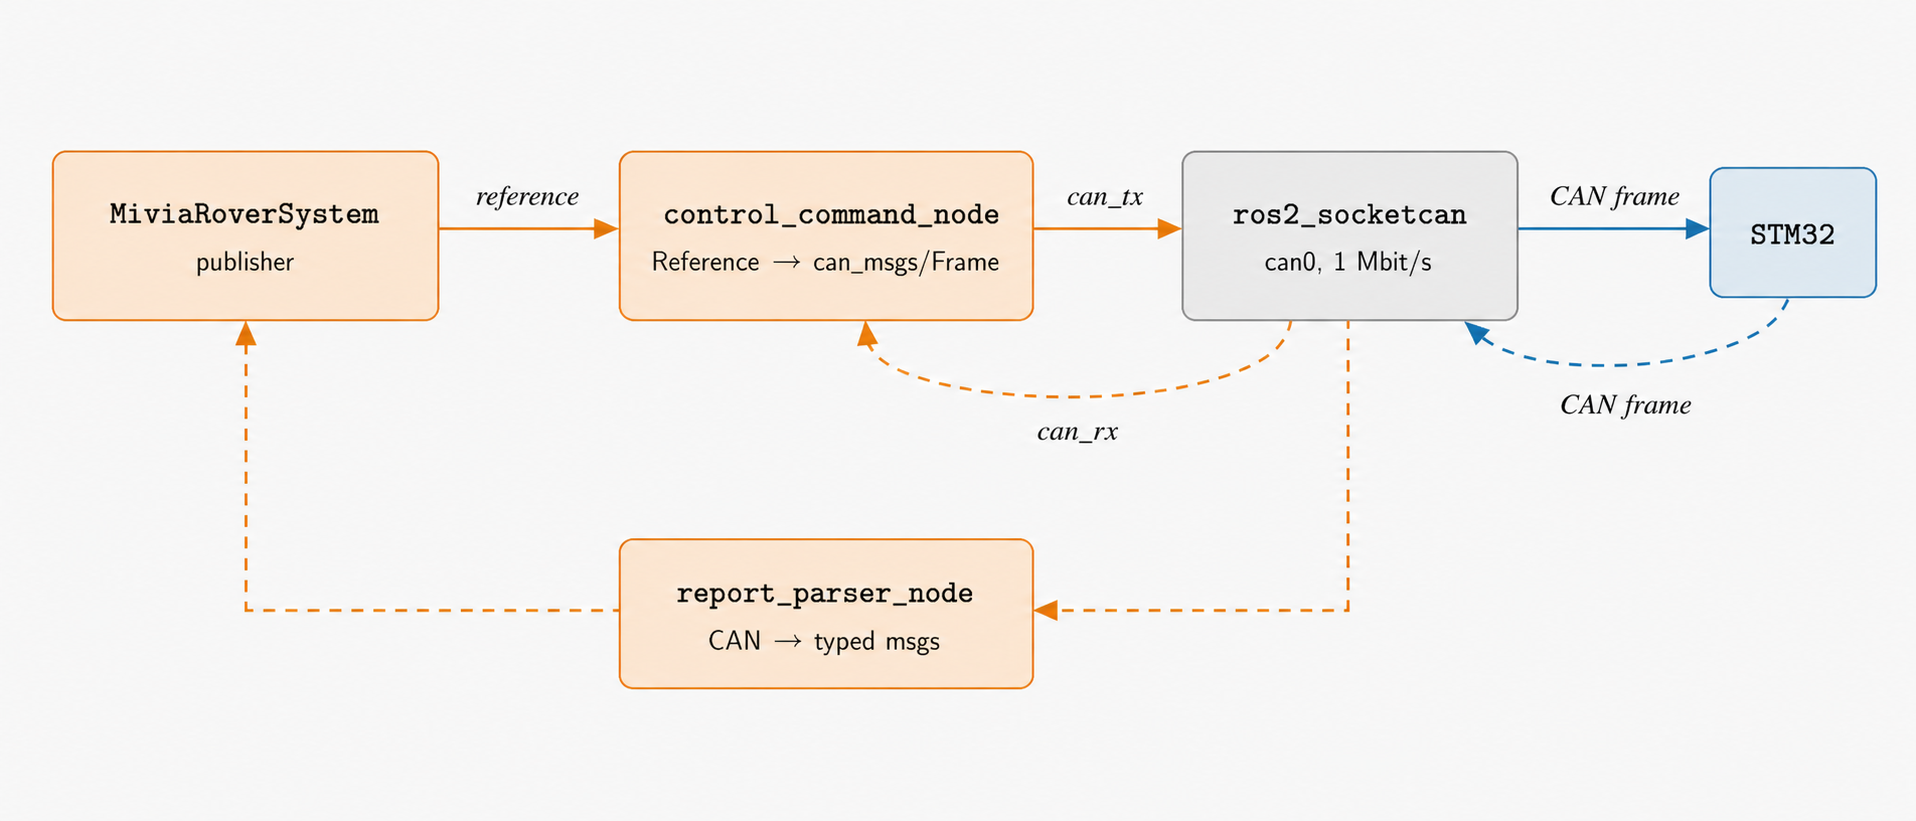
\includegraphics[width=1\textwidth,height=0.6\textheight,keepaspectratio]{images/04_ring4_can_stack.png}

  \vspace{0.4em}
  \begin{itemize}\setlength\itemsep{2pt}
    \item Three thin layers, each replaceable on its own.
    \item \texttt{ros2\_socketcan} = \emph{transport} only (no DBC
          knowledge).
    \item \texttt{control\_command} = \emph{down} serialiser — packs
          \texttt{Reference} into the \(8\)-byte packet.
    \item \texttt{report\_parser} = \emph{up} parser — switches on CAN ID and
          emits typed msgs.
  \end{itemize}
\end{frame}

% ---------------------------------------------------------------------------- %
\begin{frame}[fragile]{Ring 5 — bring-up \& launch order}
  \begin{columns}[T,onlytextwidth]
    \column{0.50\textwidth}
      \textbf{What \texttt{mivia\_rover.launch.py} does.}
      \begin{itemize}\setlength\itemsep{4pt}
        \item Builds the robot description from \texttt{xacro}.
        \item Starts \texttt{ros2\_control\_node} and
              \texttt{robot\_state\_publisher} on that same URDF.
        \item Spawns the state broadcaster, then the
              \texttt{diff\_drive\_controller}.
      \end{itemize}

      \vspace{0.6em}
      \textbf{The one important remap.}\\
      \small \texttt{/mivia\_rover\_base\_controller/cmd\_vel}\\
      \(\leftarrow\) \texttt{/cmd\_vel\_stamped}

      \vspace{0.4em}
      \footnotesize\textcolor{black!60}{That is where Nav2's smoother meets
      the base controller.}

    \column{0.50\textwidth}
      \centering
      \begin{tikzpicture}[
        node distance=4mm,
        every node/.style={font=\scriptsize},
        launchstep/.style={minimum width=58mm, minimum height=4.8mm},
        launcharr/.style={line width=0.6pt,
          -{Latex[length=1.6mm,width=1.25mm]}, shorten <=0.7mm, shorten >=0.7mm}
      ]
        \node[hl, launchstep] (a) {\texttt{xacro} renders URDF};
        \node[hl, launchstep, below=of a] (b) {\texttt{ros2\_control\_node} loads SystemInterface};
        \node[hl, launchstep, below=of b] (c) {\texttt{robot\_state\_publisher}};
        \node[hl, launchstep, below=of c] (d) {spawn \texttt{joint\_state\_broadcaster}};
        \node[hl, launchstep, below=of d] (e) {spawn \texttt{mivia\_rover\_base\_controller}};
        \node[bus, launchstep, below=of e] (f) {\texttt{mivia\_rover\_can\_bringup}};
        \node[ll, launchstep, below=of f] (g) {STM32 firmware listening on the bus};

        \draw[arrhl, launcharr] (a.south)--(b.north);
        \draw[arrhl, launcharr] (b.south)--(c.north);
        \draw[arrhl, launcharr] (c.south)--(d.north);
        \draw[arrhl, launcharr] (d.south)--(e.north);
        \draw[arrhl, launcharr] (e.south)--(f.north);
        \draw[arrll, launcharr] (f.south)--(g.north);
      \end{tikzpicture}\\[3pt]
      \scriptsize\textcolor{black!60}{In the bringup orchestrator, platform
      and CAN are toggled independently — handy during validation.}
  \end{columns}
\end{frame}

% ---------------------------------------------------------------------------- %
\begin{frame}{Take-aways from Atto~4}
  \begin{enumerate}\setlength\itemsep{2pt}
    \item \textbf{Five rings, no magic.} From \texttt{cmd\_vel} to a CAN
          frame, every step is a small, named piece you can read in one
          sitting.
    \item \textbf{The contract is set in the URDF}: four \texttt{velocity}
          command interfaces, four \texttt{position+velocity} state
          interfaces. The rest is implementation detail.
    \item \textbf{Real-time discipline} lives in the SystemInterface:
          double-buffered commands, a NON-RT comm thread, a publisher that
          \emph{always} ticks — even on fault.
    \item \textbf{ROS handles the bus too.} \texttt{ros2\_socketcan} +
          \texttt{control\_command} + \texttt{report\_parser} = three
          replaceable layers; the platform package never opens a socket.
  \end{enumerate}
\end{frame}
